\documentclass{article}
\usepackage[utf8]{inputenc}
\usepackage{listings}
\usepackage{cite}
\usepackage{amsmath,amssymb,amsfonts}
\usepackage{algorithmic}
\usepackage{graphicx}
\usepackage{textcomp}
\usepackage{xcolor}
\usepackage{color}
\usepackage{url}
\definecolor{dkgreen}{rgb}{0,0.6,0}
\definecolor{gray}{rgb}{0.5,0.5,0.5}
\definecolor{mauve}{rgb}{0.58,0,0.82}
\lstset{%
    aboveskip=3mm, belowskip=3mm,
    showstringspaces=false,
    columns=flexible,
    basicstyle={\small\ttfamily},
    numbers=none,
    numberstyle=\tiny\color{red},
    keywordstyle=\color{blue},
    commentstyle=\color{dkgreen},
    stringstyle=\color{mauve},
    breaklines=true,
    breakatwhitespace=true,
    tabsize=3
}

\newcommand{\code}[1]{\texttt{#1}}
\newcommand{\val}[1]{#1_{\text{val}}}
\newcommand{\est}[1]{#1_{\text{est}}}

\begin{document}
\title{Lab 1 --- Fundamental Signal Processing}
\author{Malcolm Vigren, \textit{malvi108} \\
        Emil Segerbäck, \textit{emise935}}

\maketitle

Inställningar för 1:
numHidden = 8
numIterations = 1000
learningRate = 0.001

\section{Overview}
Dataset 1 can be classified using a linear classifier. However, the
other datasets are not linearly separable.

\section{Downsampling}
Downsampling the data removes noise from the images which prevents the
network from trying to learn the noise.

\section{kNN}
We used the \texttt{mink} function in matlab to find the closest k
data points and then we use \texttt{mode} to check for the most
frequent kind.

\section{Draws in kNN}
Because \texttt{mode} returns the smallest element in a case of a tie
that will also happen to our algorithm.

\section{Selection of best k}
We looped for all k between 1 and 100 and checked for which values it
worked best.

\section{Backpropagation}
\subsection{Single layer}

The gradient of the cost function was evaluated to

\begin{equation}
  \frac{\partial \epsilon}{\partial w_{ij}} =
  \frac{\partial \epsilon}{\partial z_j}
  \frac{\partial z_j}{\partial s_j}
  \frac{\partial s_j}{\partial w_{ij}}
\end{equation}

where $s_j$ is

\begin{equation}
  s_j = \sum_{k}{w_{kj}h_k}
\end{equation}

and $z_j = s_j$, since we don't use an activation function.
The partial derivatives were evaluated to

\begin{equation}
    \frac{\partial \epsilon}{\partial z_j} = 2\sum_j(y_j - z_j)
\end{equation}

\begin{equation}
    \frac{\partial z_j}{\partial s_j} = 1
\end{equation}

\begin{equation}
    \frac{\partial s_j}{\partial w_{ij}} = h_i
\end{equation}

\subsubsection{Multi layer}

The gradient of the weights of the output layer was evaluated as:

\begin{equation}
  \frac{\partial \epsilon}{\partial w_{ij}} =
  \frac{\partial \epsilon}{\partial z_j}
  \frac{\partial z_j}{\partial s_j}
  \frac{\partial s_j}{\partial w_{ij}}
\end{equation}

This is similar to the gradient in the single-layer-network, where $h_i$
in the last partial derivative is replaced with the output from the hidden
layer:

\begin{equation}
    \frac{\partial s_j}{\partial w_{ij}} = \sigma(a_j)
\end{equation}

where $a_j$ is 

\begin{equation}
    a_j = \sum_{n=1}^Q v_{jn}h_n
\end{equation}

The gradient of the hidden layer was evaluated as follows:

\begin{equation}
  \frac{\partial \epsilon}{\partial v_{jn}} =
  \frac{\partial \epsilon}{\partial z_m}
  \frac{\partial z_m}{\partial s_m}
  \frac{\partial s_m}{\partial q_j}
  \frac{\partial q_j}{\partial a_j}
  \frac{\partial a_j}{\partial v_{jn}}
\end{equation}

where $q_j = \sigma(a_j)$.

\section{Training}

\subsection{Dataset 1}

We chose the single-layer network for dataset 1, since this 
is easily linearly separable. We used 200 iterations and a learning rate of
0.0001. Figure~\ref{fig:res1} shows the result of this.

\begin{figure}
    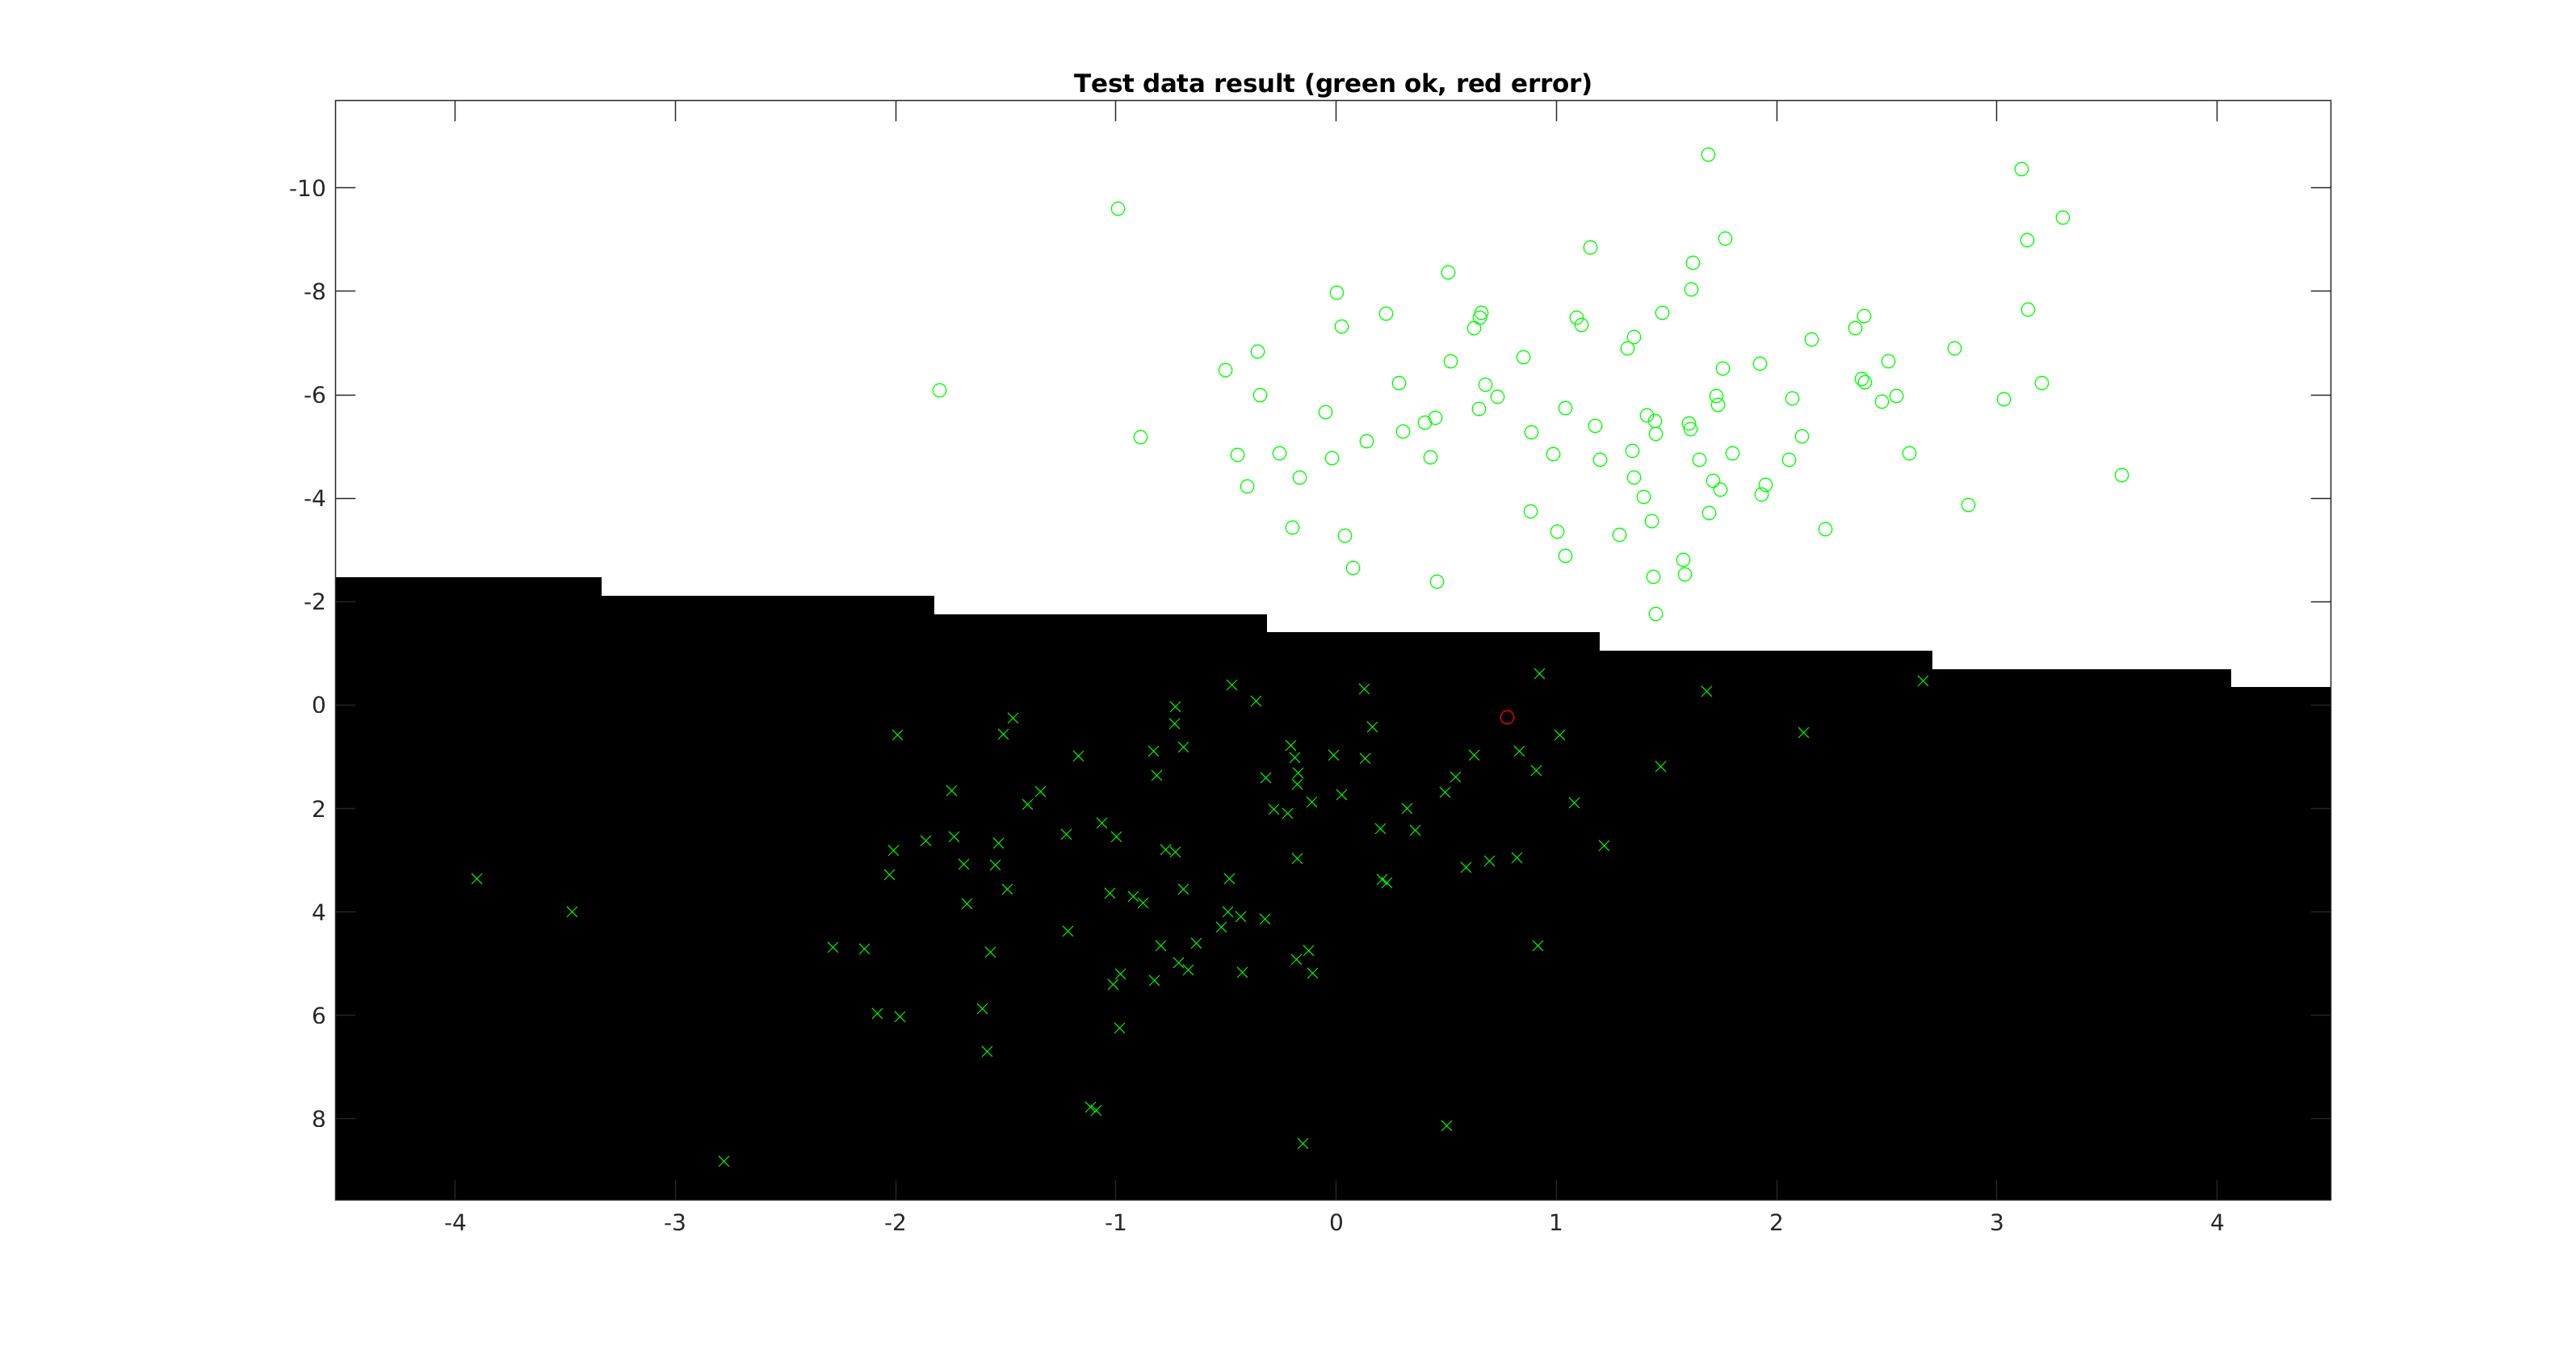
\includegraphics[width=13cm]{dataset1res.png}
    \caption{Results for dataset 1}
    \label{fig:res1}
\end{figure}

\subsection{Dataset 2}

Here we used the multilayer network with 10 hidden neurons, 4000 iterations and a
learning rate of 0.002. A multilayer network is required here, since the data
is not linearly separable with only 2 dimensions. Having more hidden neurons
than input neurons increases the dimensionality of the problem, making it
possible to separate the classes.

The exact parameters were found through trial and error. They were chosen such
that we got high accuracy without taking too long to train.

\begin{figure}
    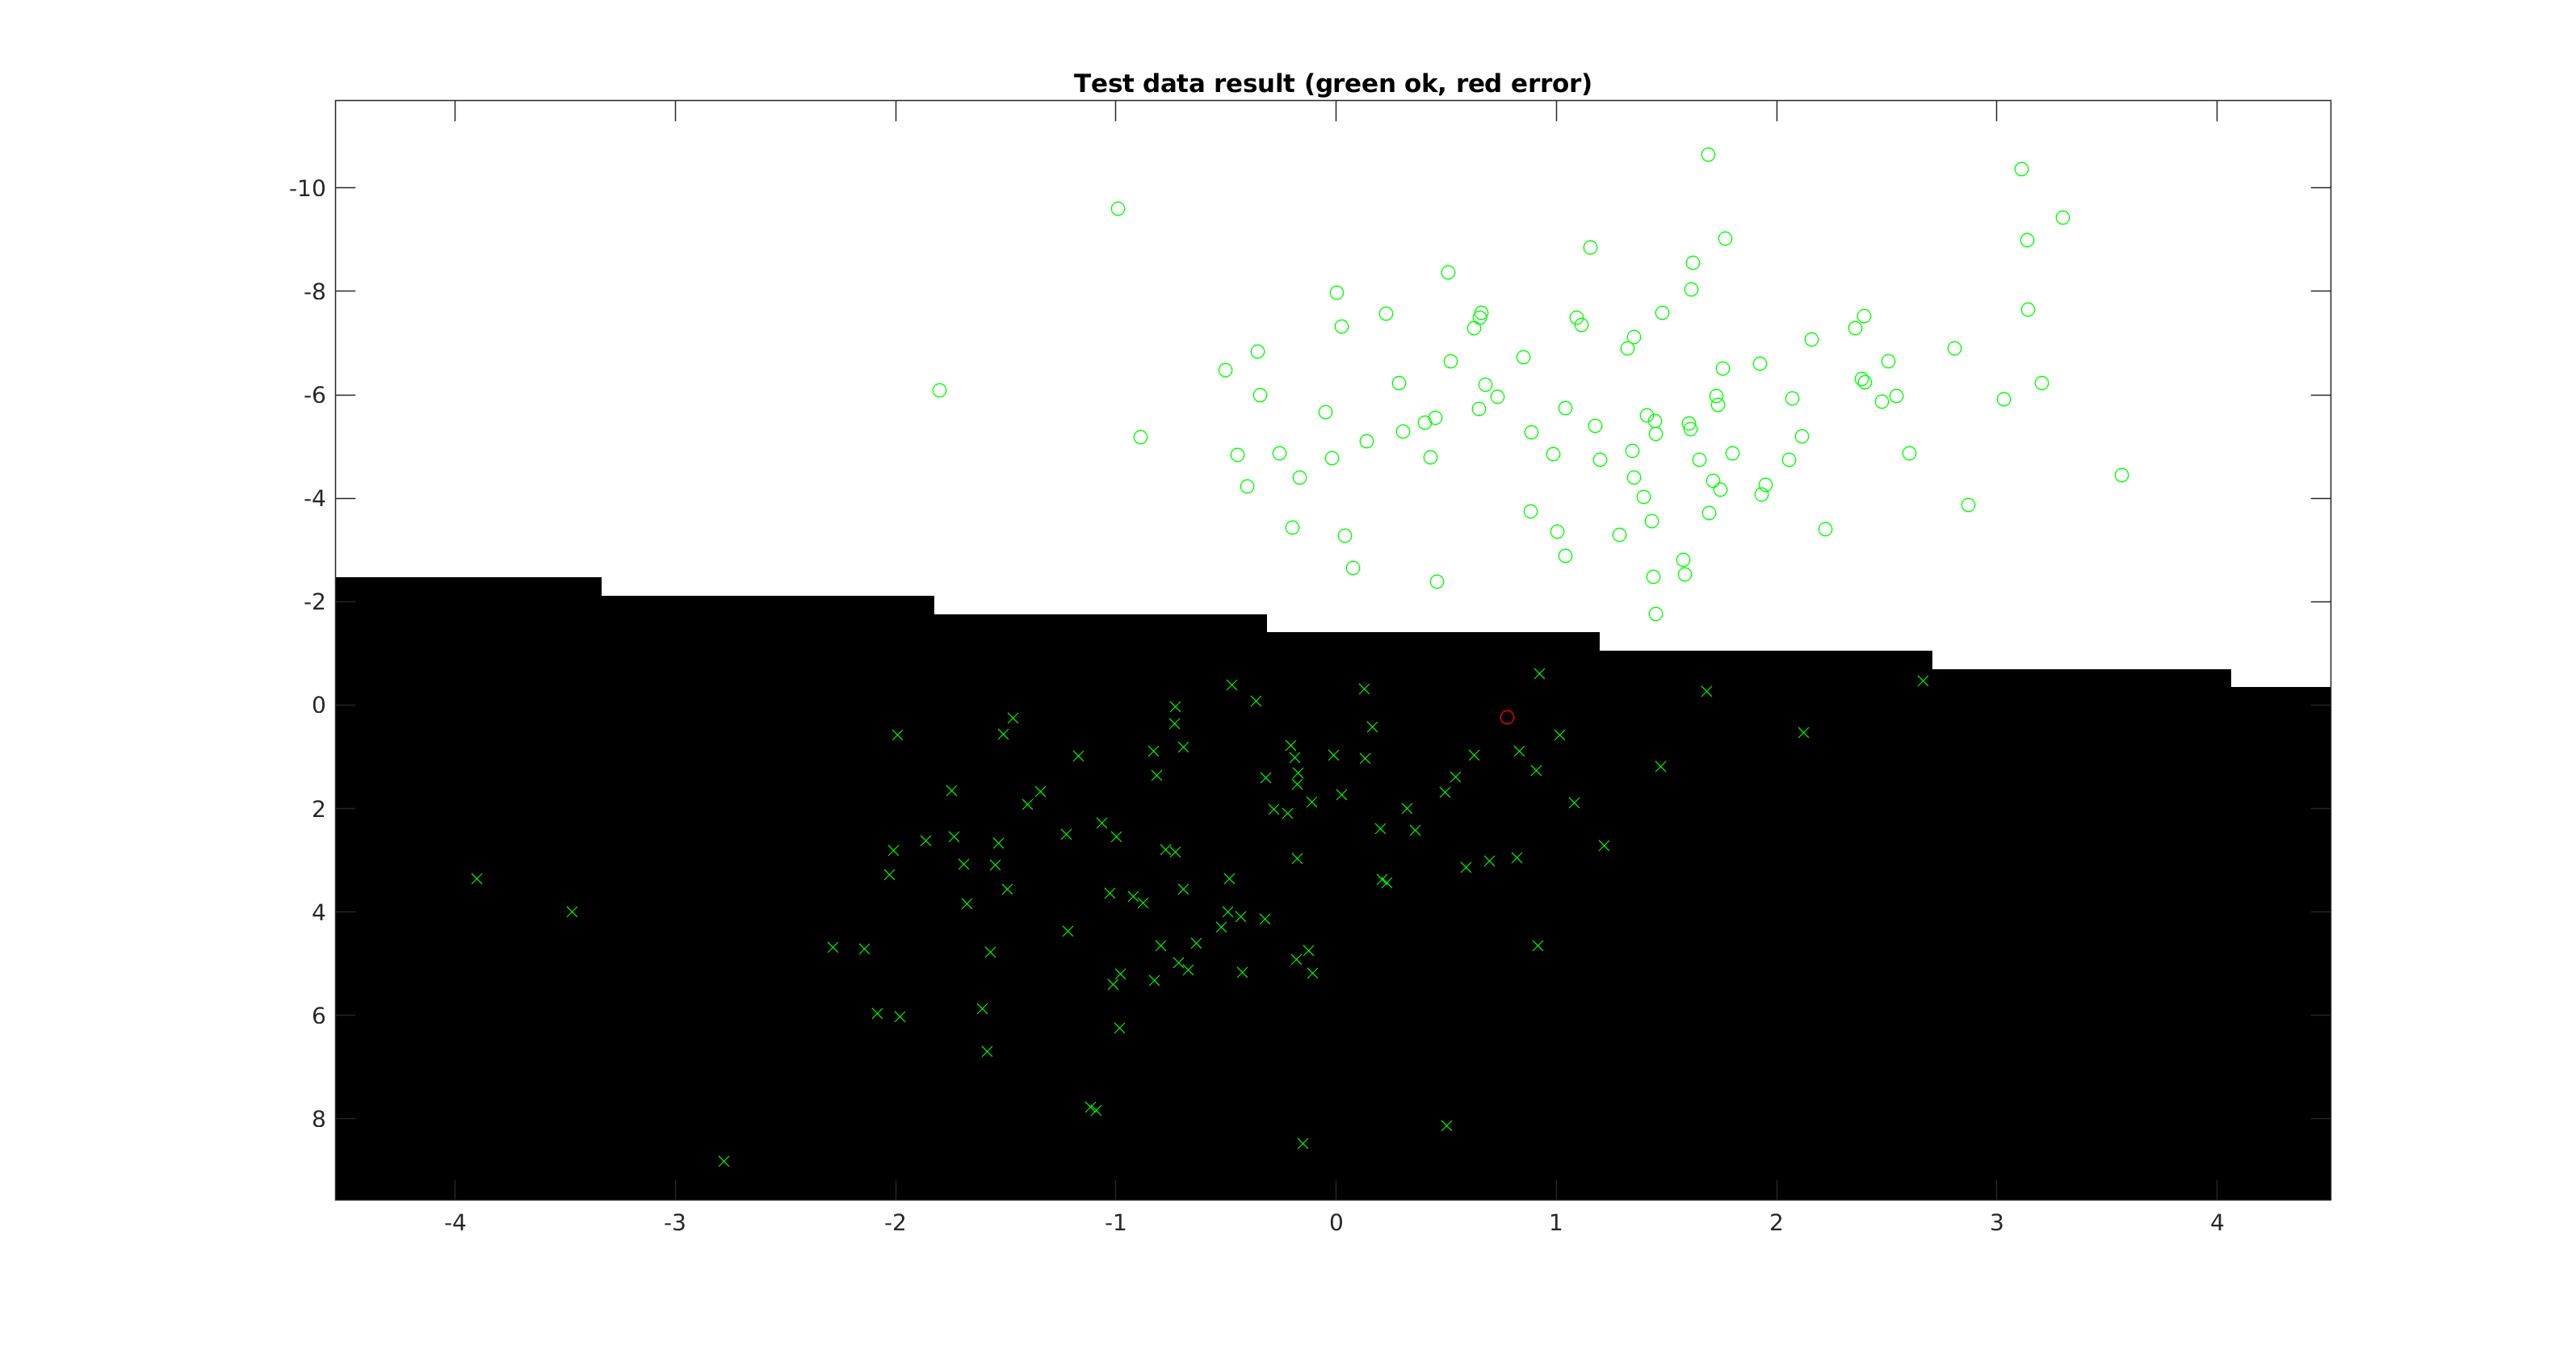
\includegraphics[width=13cm]{dataset1res.png}
    \caption{Results for dataset 2}
    \label{fig:res1}
\end{figure}

For the other datasets we chose a multi layer network because they
require a non linear classifier.

Inställningar för 2:
numHidden = 10
numIterations = 4000
learningRate = 0.002

Inställningar för 3:
numHidden = 16
numIterations = 1200
learningRate = 0.004

Inställningar för 4:
numHidden = 100
numIterations = 4000
learningRate = 0.004

\subsection{Dataset 3}
\subsection{Dataset 4}

\subsection{Solution}

\section{Discussion}

\section{Improvements}

\end{document}
